% Generated from ../answer.md with the classroom-report LaTeX template.
\documentclass[12pt,a4paper,fontset=none]{ctexart}

\usepackage[left=2.7cm,right=2.7cm,top=2.5cm,bottom=2.5cm]{geometry}
\usepackage{amsmath, amssymb}
\usepackage{booktabs}
\usepackage{longtable}
\usepackage{array}
\usepackage{calc}
\usepackage[font=small,labelfont=bf,labelsep=quad]{caption}
\usepackage{graphicx}
\usepackage{float}
\usepackage{hyperref}
\usepackage{xurl}
\usepackage{xcolor}
\usepackage{fancyvrb}
\usepackage{fvextra}
\usepackage{setspace}
\usepackage{enumitem}
\usepackage{etoolbox}

\let\OriginalIncludeGraphics\includegraphics
\renewcommand{\includegraphics}[2][]{%
  \OriginalIncludeGraphics[width=\linewidth,height=0.88\textheight,keepaspectratio,#1]{#2}%
}

\setmainfont{Noto Serif CJK SC}
\setCJKmainfont{Noto Serif CJK SC}
\setmonofont[Scale=0.9]{DejaVu Sans Mono}
\setCJKmonofont[Scale=0.9]{Noto Sans CJK SC}
\graphicspath{{../}{../assets/}{../../../result/}{../../../results/}{../../../outputs/}}
\setstretch{1.36}
\AtBeginDocument{\zihao{-4}\selectfont}
\setlength{\parindent}{2em}
\setlength{\parskip}{0pt}
\setlength{\abovedisplayskip}{0.65\baselineskip}
\setlength{\belowdisplayskip}{0.65\baselineskip}
\captionsetup{skip=0.35\baselineskip}
\sloppy
\clubpenalty=10000
\widowpenalty=10000

\hypersetup{hidelinks}

\setcounter{secnumdepth}{3}
\setcounter{tocdepth}{2}
\renewcommand{\thesubsection}{\arabic{subsection}}
\renewcommand{\thesubsubsection}{\thesubsection.\arabic{subsubsection}}
\ctexset{
  section = {
    format = {\centering\zihao{4}\bfseries},
    aftername = {\quad},
    beforeskip = {1.1\baselineskip},
    afterskip = {0.65\baselineskip}
  },
  subsection = {
    format = {\zihao{-3}\bfseries},
    aftername = {\quad},
    beforeskip = {1.0\baselineskip},
    afterskip = {0.45\baselineskip}
  },
  subsubsection = {
    format = {\zihao{4}\bfseries},
    aftername = {\quad},
    beforeskip = {0.75\baselineskip},
    afterskip = {0.25\baselineskip}
  }
}

\newcommand{\reportgroup}[1]{%
  \phantomsection\addcontentsline{toc}{section}{#1}%
  \begin{center}
    {\zihao{4}\bfseries #1\par}%
  \end{center}
  \vspace{0.65\baselineskip}%
}
\newcommand{\problem}[1]{\subsection{#1}}
\newcommand{\blocktitle}[1]{\subsubsection{#1}}
\newcommand{\analysispart}[1]{\par\medskip\noindent{\bfseries #1}\par\nobreak\smallskip}
% 标题层级规则：
% 1. \reportgroup 用于罗马编号的大组标题，例如“I. 数值方法误差分析”；它只写入目录，不占用 subsection 编号。
% 2. \problem 用于真正的题目或小问标题，例如“Problem 1(a)：公式推导与算法设计”；它对应 subsection 编号。
% 3. \blocktitle 用于题内固定小节，例如“待求问题”“解决方式”“问题答案”“分析”。
% 4. 若一个大组下有背景介绍和多个小问，不要额外写 \textbf{Problem 1：...} 或另造标题宏；
%    直接在 \reportgroup 后写普通介绍段，再进入 \problem。
% 示例：
% \reportgroup{I. Gregory-Leibniz 级数计算圆周率}
% 本节利用 Gregory-Leibniz 级数计算 \(\pi\)。
% \problem{Problem 1(1)：有限项计算}
% \scriptlink{problem1.c}
% 内联排版规则：
% 1. 正文内的英文、数字、短命令和路径应尽量保持同一正文字体，避免一段内混用多套字形。
% 2. \codeinline 只提供内联技术词标记，不切换到等宽字体；真正的命令片段放入 CodeBlock。
% 3. 普通数值和单位不要用 \texttt；直接使用正文，例如 3734 km/s。
% 4. 文件路径使用 \fileinline；它保持正文字体，并使用 URL 断行规则，避免长路径拉坏行距。
% 5. 正文公式、变量、等式和指数必须使用数学模式，例如 \(2^{-10}\)、\(1+t\)、\((1+t)^2-1\)、\(b=100\)；
%    不要写成 \texttt{2\^{}(-10)}、\texttt{1+t} 或 \texttt{(1+t)\^{}2-1}，否则只会按代码文本排版。
\newcommand{\codeinline}[1]{{\normalfont #1}}
\newcommand{\fileinline}[1]{{\urlstyle{same}\nolinkurl{#1}}}
\newcommand{\scriptpath}[1]{\fileinline{#1}}
\newcommand{\githubscriptsbase}{https://github.com/Void0312Aurora/computational-physics-homework-2026/blob/main/04/scripts}
\newcommand{\scriptlink}[1]{\noindent\textbf{相关脚本：}\href{../../../scripts/#1}{本地 \scriptpath{scripts/#1}} / \href{\githubscriptsbase/#1}{GitHub \scriptpath{scripts/#1}}\par\medskip}

\DefineVerbatimEnvironment{verbatim}{Verbatim}{
  fontsize=\footnotesize,
  frame=single,
  framesep=0.5em,
  xleftmargin=1.2em,
  xrightmargin=1.2em,
  breaklines=true,
  breakanywhere=true
}
\DefineVerbatimEnvironment{CodeBlock}{Verbatim}{
  fontsize=\footnotesize,
  frame=single,
  framesep=0.5em,
  xleftmargin=1.2em,
  xrightmargin=1.2em,
  breaklines=true,
  breakanywhere=true
}
\providecommand{\tightlist}{\setlength{\itemsep}{0pt}\setlength{\parskip}{0pt}}
\providecommand{\pandocbounded}[1]{#1}
\newcounter{none}
\newcommand{\passthrough}[1]{#1}
\setlist{nosep,leftmargin=2em}
\setlength{\LTpre}{0.35\baselineskip}
\setlength{\LTpost}{0.35\baselineskip}
\newif\ifwidetable
\newif\iftighttable
\setlength{\tabcolsep}{4pt}
\AtBeginEnvironment{longtable}{%
  \iftighttable
    \fontsize{6.7pt}{8.1pt}\selectfont\setlength{\tabcolsep}{0pt}%
  \else\ifwidetable
    \footnotesize\setlength{\tabcolsep}{2pt}%
  \else
    \normalsize\setlength{\tabcolsep}{4pt}%
  \fi\fi
  \renewcommand{\arraystretch}{1.16}%
}
\emergencystretch=3em

\title{\vspace{-1.0em}{\bfseries\zihao{3} Homework 5}\\[0.35em]{\zihao{-4} 非线性方程与复平面迭代实验报告}}
\author{\zihao{-4} 姜玥晟、周鑫志、高西飞}
\date{\zihao{-4} 2026-04-22}

\begin{document}
\pagestyle{plain}
\maketitle

\begin{figure}[H]
  \centering
  \begin{minipage}[t]{0.30\linewidth}
    \centering
    
\includegraphics[width=0.72\linewidth,height=0.22\textheight,keepaspectratio]{../assets/pic_1.jpg}\\[0.35em]
    姜玥晟
  \end{minipage}\hfill
  \begin{minipage}[t]{0.30\linewidth}
    \centering
    
\includegraphics[width=0.72\linewidth,height=0.22\textheight,keepaspectratio]{../assets/pic_2.jpg}\\[0.35em]
    周鑫志
  \end{minipage}\hfill
  \begin{minipage}[t]{0.30\linewidth}
    \centering
    
\includegraphics[width=0.72\linewidth,height=0.22\textheight,keepaspectratio]{../assets/pic_3.jpg}\\[0.35em]
    高西飞
  \end{minipage}
\end{figure}

\begin{table}[H]
  \centering
  \begin{tabular}{p{0.22\linewidth}p{0.68\linewidth}}
    \toprule
    项目 & 内容 \\
    \midrule
    源题编号 & \codeinline{HW05} \\
    作业属性 & 小组作业 \\
    小组成员 & 姜玥晟、周鑫志、高西飞 \\
    报告主题 & Newton/Secant 分形、混合求根、Brent 型算法、范盛金公式与地月系统 \(L_1\) 点 \\
    实验环境 & \codeinline{Python} 数值程序、\codeinline{mpmath} 参考值与图像后处理；Problem 1 主结果由多进程 CPU 程序生成 \\
    \bottomrule
  \end{tabular}
\end{table}

\newpage
\renewcommand{\contentsname}{目录}
\begingroup
\hypersetup{linkcolor=black}
\tableofcontents
\thispagestyle{plain}
\endgroup
\newpage

\reportgroup{I. 三次方程的 Newton 与 Secant 分形}

\problem{Problem 1：三次方程的 Newton 与 Secant 分形}

\scriptlink{problem1.py}

\blocktitle{待求问题}

对复方程

\[
f(z)=z^3-1=0
\]

使用 Newton-Raphson 方法生成分形图，并调节合适的收敛容差。题目还要求提供两套配色方案；可选部分要求改用 secant 方法并讨论是否仍能观察到分形结构。

\blocktitle{解决方式}

Newton 分形的计算流程如下：

\begin{CodeBlock}
Input : complex grid G, tolerance tau, max_iter K
Output: basin label and iteration count

roots <- {1, exp(2pi i / 3), exp(4pi i / 3)}
for each z0 in G do
    z <- z0
    for k from 1 to K do
        z <- z - (z^3 - 1) / (3 z^2)
        if min_j |z - roots[j]| < tau then
            record basin j and iteration k
            break
        end if
    end for
    if no convergence then
        mark point as unconverged
    end if
end for
render two color maps from the same basin data
\end{CodeBlock}

可选 secant 版本则把单点迭代改为双点迭代

\[
z_{n+1}=z_n-\frac{f(z_n)(z_n-z_{n-1})}{f(z_n)-f(z_{n-1})},
\]

并取 \(z_1=z_0+(0.2+0.2i)\) 作为第二初值。

\blocktitle{问题答案}

本次主流程采用收敛容差

\[
\tau=5\times 10^{-7}.
\]

在这一设置下，Newton 与 secant 的主结果如图 1 所示。

\begin{figure}
\centering
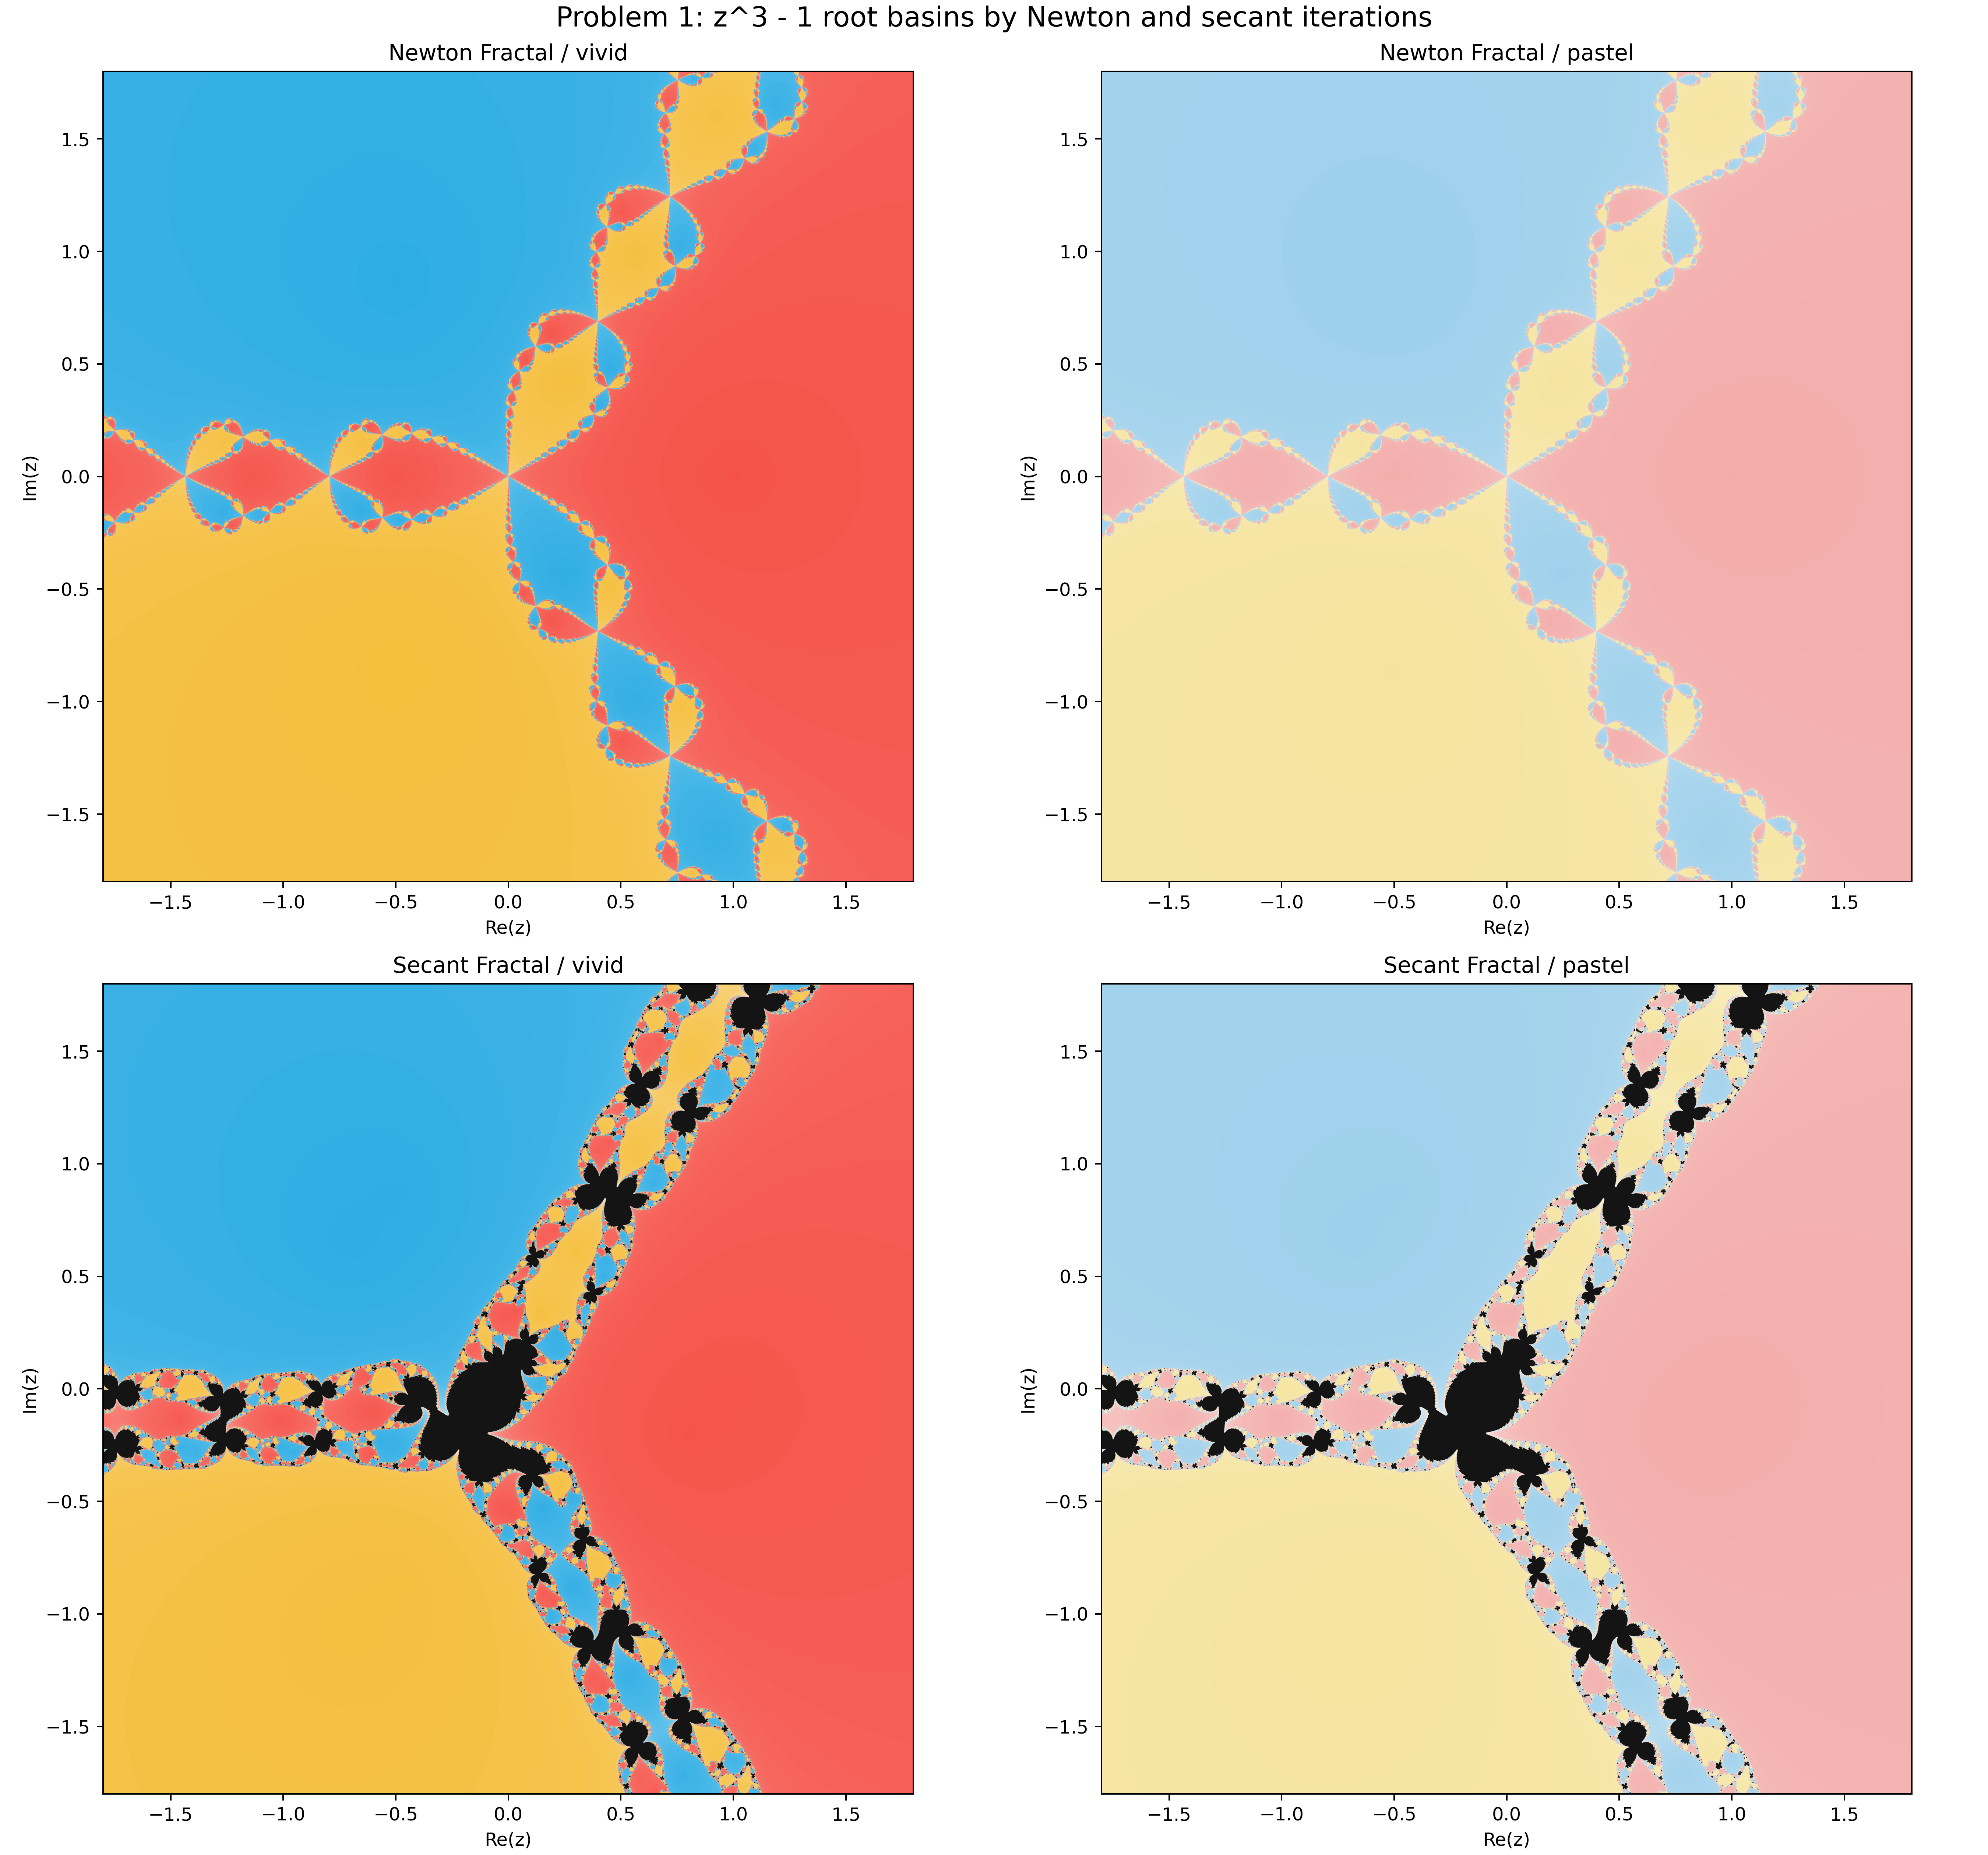
\includegraphics[width=0.92\linewidth,height=0.78\textheight,keepaspectratio,alt={Problem 1 Fractals}]{../../../result/problem1_fractals.png}
\caption{Problem 1 Fractals}
\end{figure}

统计结果见表 1。

{\def\LTcaptype{none} % do not increment counter
\widetabletrue
\begin{longtable}[]{@{}
  >{\raggedright\arraybackslash}p{(\linewidth - 10\tabcolsep) * \real{0.1667}}
  >{\raggedleft\arraybackslash}p{(\linewidth - 10\tabcolsep) * \real{0.1667}}
  >{\raggedleft\arraybackslash}p{(\linewidth - 10\tabcolsep) * \real{0.1667}}
  >{\raggedleft\arraybackslash}p{(\linewidth - 10\tabcolsep) * \real{0.1667}}
  >{\raggedleft\arraybackslash}p{(\linewidth - 10\tabcolsep) * \real{0.1667}}
  >{\raggedleft\arraybackslash}p{(\linewidth - 10\tabcolsep) * \real{0.1667}}@{}}
\toprule\noalign{}
\begin{minipage}[b]{\linewidth}\raggedright
方法
\end{minipage} & \begin{minipage}[b]{\linewidth}\raggedleft
收敛比例
\end{minipage} & \begin{minipage}[b]{\linewidth}\raggedleft
平均迭代步数
\end{minipage} & \begin{minipage}[b]{\linewidth}\raggedleft
root 1 占比
\end{minipage} & \begin{minipage}[b]{\linewidth}\raggedleft
root 2 占比
\end{minipage} & \begin{minipage}[b]{\linewidth}\raggedleft
root 3 占比
\end{minipage} \\
\midrule\noalign{}
\endhead
\bottomrule\noalign{}
\endlastfoot
Newton & 0.9999997275 & 6.8145 & 0.341879 & 0.329060 & 0.329060 \\
Secant & 0.9452318 & 9.1147 & 0.359842 & 0.315501 & 0.269889 \\
\end{longtable}
}

据此可以直接回答题目三点要求：

\begin{enumerate}
\def\labelenumi{\arabic{enumi}.}
\tightlist
\item
  取 \(5\times 10^{-7}\) 作为容差时，Newton 分形边界已经清晰可辨，能够兼顾图像效果与计算成本。
\item
  两套配色方案已经输出到同一张主图中，满足题面要求。
\item
  secant 方法仍然能够观察到分形结构，但其未收敛区域更多、平均步数更大：在 \(20000\times 20000\) 主网格上，secant 的未收敛点约为 \(21907280\) 个，是 Newton 的约 \(2.01\times 10^5\) 倍；其平均迭代步数也比 Newton 高 \(33.75\%\)。因此，secant 的稳定性和收敛效率均弱于 Newton 方法。
\end{enumerate}

\blocktitle{分析}

本节聚焦 Problem 1 的主体数值问题：在同一复平面采样范围和同一收敛容差下，比较 Newton 与 secant 迭代的分形结构、收敛效率和稳定性。为避免把性能工程内容混入方法分析，CPU 并行剖面、CPU ultra 与 GPU/精度扩展统一放在后面的``扩展''小节。

本题最先完成的是纯 CPU 主流程，而不是 GPU 路线。\codeinline{solution.py} 使用 \codeinline{ProcessPoolExecutor} 按行带切分复平面，先在 \(20000\times 20000\) 计算网格上完成 Newton 与 secant 迭代，再降采样得到 \(5000\times 5000\) 的交付图像。表 1 与图 1 的全部结果都来自这条 CPU 实现链。

就主实验而言，Newton 与 secant 都在复平面上定义了高度非线性的迭代映射，因此都会在根吸引域交界处形成分形边界。二者的差别不在于``是否存在分形''，而在于 secant 使用双初值且不显式调用导数，因此收敛域更易破碎，平均迭代步数也更大。对应地，在 80 个 worker 的 CPU 基线运行中，Newton 的收敛比例达到 \(0.9999997275\)，平均迭代步数为 \(6.8145\)；secant 的收敛比例为 \(0.9452318\)，平均迭代步数增至 \(9.1147\)。CPU 基线总耗时为 231.04 s，峰值内存约 98.71 GiB，说明当采样网格极大时，主流程的首要压力来自全局数组规模。

更严格地说，本题的定量分析应先从误差模型开始。设目标根为 \(\alpha\)，满足 \(\alpha^3=1\)，并记局部误差为
\[
e_n=z_n-\alpha .
\]
Newton 迭代在单根附近满足标准 Taylor 展开
\[
e_{n+1}
=\frac{f''(\alpha)}{2f'(\alpha)}e_n^2+O(e_n^3)
=\alpha^{-1}e_n^2+O(e_n^3).
\]
由于三个根都满足 \(|\alpha|=1\)，主导系数的模为 1，因此 Newton 的局部误差近似满足 \(|e_{n+1}|\approx |e_n|^2\)，收敛阶为 2。secant 方法的局部误差递推则为
\[
e_{n+1}
=\frac{f''(\alpha)}{2f'(\alpha)}e_ne_{n-1}
 +O(e_ne_{n-1}(e_n+e_{n-1}))
=\alpha^{-1}e_ne_{n-1}+O(e_ne_{n-1}(e_n+e_{n-1})).
\]
若令渐近收敛阶为 \(p\)，则有 \(p^2=p+1\)，即
\[
p=\frac{1+\sqrt{5}}{2}\approx 1.618 .
\]
这一局部模型给出第一条可检验预期：当迭代轨道已经进入某个根的局部吸引区后，secant 仍应当收敛，但其阶数低于 Newton，因此平均迭代步数和高分位迭代步数应系统性更大。

第二层模型是全局稳定性。Newton 是单状态映射
\[
N(z)=z-\frac{z^3-1}{3z^2},
\]
其主要奇异性来自 \(z=0\) 处的导数分母。secant 则是双状态映射
\[
S(z_{n-1},z_n)
=z_n-\frac{(z_n^3-1)(z_n-z_{n-1})}{z_n^3-z_{n-1}^3}.
\]
利用恒等式 \(a^3-b^3=(a-b)(a^2+ab+b^2)\)，在第一步 \(z_1=z_0+\delta\) 时可写成
\[
z_2
=z_1-\frac{z_1^3-1}{z_1^2+z_1z_0+z_0^2}.
\]
因此 secant 的有效分母为
\[
D_0=z_1^2+z_1z_0+z_0^2 .
\]
当 \(|D_0|\) 很小时，secant 步长及其对 \(z_0\)、\(\delta\) 的扰动响应都会被放大；轨道可能跨越吸引域边界，或者在最大迭代步数内不能进入任一根的局部收敛区。这给出另外两条可检验预期：其一，secant 的未收敛比例和失效邻域比例应显著高于 Newton；其二，改变第二初值偏移 \(\delta\) 会改变吸引域划分，即使两个设置都收敛，也可能收敛到不同的根。

把主实验统计量换成失败概率后，secant 的不稳定性可以更直接地量化。\((20000\times 20000)\) 主网格共有 \(4.0\times 10^8\) 个初值，Newton 的未收敛比例仅为 \(2.725\times 10^{-7}\)，约对应 109 个采样点；secant 的未收敛比例为 \(5.47682\times 10^{-2}\)，约对应 21907280 个采样点。换言之，在同一容差和同一复平面范围内，secant 的失败概率约为 Newton 的 \(2.0098\times 10^5\) 倍；其平均迭代步数比 Newton 多 2.3002 步，相对增加 \(33.75\%\)。因此，``secant 更不稳定''不是仅由图像观感得到的定性判断，而是同时体现在失败率和收敛速度两个指标上。

{\def\LTcaptype{none} % do not increment counter
\begin{longtable}[]{@{}lrr@{}}
\toprule\noalign{}
主网格指标 & Newton & Secant \\
\midrule\noalign{}
\endhead
\bottomrule\noalign{}
\endlastfoot
计算网格点数 & 400000000 & 400000000 \\
未收敛比例 & \(2.725\times 10^{-7}\) & \(5.47682\times 10^{-2}\) \\
估计未收敛点数 & 109 & 21907280 \\
平均迭代步数 & 6.8145 & 9.1147 \\
相对 Newton 的平均步数 & 1.0000 & 1.3375 \\
\end{longtable}
}

为了进一步区分``收敛慢''和``分类敏感''两类现象，又补充了一个 \(1024\times 1024\) 的轻量稳定性扫描，脚本为 \fileinline{scripts/problem1_secant_stability.py}，结果保存在 \fileinline{result/analysis/problem1_secant_stability_summary.csv} 和 \fileinline{result/analysis/problem1_secant_delta_sensitivity.csv}。这里没有重新运行昂贵的 \(20000\times 20000\) 主实验，而是用同一容差、同一迭代上限和同一复平面范围复核局部统计。邻域根标签翻转率定义为：在水平或竖直相邻且均已收敛的像素对中，二者收敛到不同根的比例；失效邻域对比例定义为：相邻像素对中至少一个像素未收敛的比例。

{\def\LTcaptype{none} % do not increment counter
\widetabletrue
\begin{longtable}[]{@{}lrr@{}}
\toprule\noalign{}
\(1024^2\) 稳定性指标 & Newton & Secant, \(\delta=0.2+0.2i\) \\
\midrule\noalign{}
\endhead
\bottomrule\noalign{}
\endlastfoot
收敛比例 & 0.99999809 & 0.94532776 \\
未收敛比例 & \(1.907\times 10^{-6}\) & \(5.46722\times 10^{-2}\) \\
平均迭代步数 & 6.8144 & 9.1196 \\
\(p95\) 迭代步数 & 13 & 18 \\
\(p99\) 迭代步数 & 19 & 28 \\
邻域根标签翻转率 & 0.01695 & 0.02083 \\
失效邻域对比例 & \(3.82\times 10^{-6}\) & 0.06133 \\
\end{longtable}
}

这组轻量复核与主网格统计保持一致：secant 的收敛率仍约为 0.945，而 Newton 接近全域收敛。更细地看，secant 的 \(p99\) 迭代步数达到 28，比 Newton 的 19 多 9 步；失效邻域对比例达到 0.06133，说明未收敛点不是少量孤立异常，而是在局部区域内形成可见的失效带或失效斑块。邻域根标签翻转率从 Newton 的 0.01695 增至 secant 的 0.02083，也表明 secant 的吸引域边界更碎，局部初值扰动更容易跨入不同根的吸引域。

secant 的另一类敏感性来自第二初值的选取。主程序默认取 \(z_1=z_0+(0.2+0.2i)\)；在轻量扫描中，将偏移量改为 \(0.1+0.1i\)、\(0.3+0.3i\)、\(0.2+0.0i\) 和 \(0.0+0.2i\) 后，收敛比例在 0.94311619 到 0.94785309 之间变化，跨度约 0.004737，即 0.47 个百分点。更重要的是，在与默认偏移共同收敛的采样点中，最终根标签仍有 \(8.63\%\) 到 \(10.10\%\) 发生改变；这说明 secant 的双初值设置会实质性改变吸引域划分，而不仅仅改变迭代耗时。

{\def\LTcaptype{none} % do not increment counter
\widetabletrue
\begin{longtable}[]{@{}lrrr@{}}
\toprule\noalign{}
Secant 第二初值偏移 \(\delta\) & 收敛比例 & 相对默认偏移的收敛变化 & 共同收敛点的根标签不一致比例 \\
\midrule\noalign{}
\endhead
\bottomrule\noalign{}
\endlastfoot
\(0.2+0.2i\) & 0.94532776 & 0.000000 & 0.00000 \\
\(0.1+0.1i\) & 0.94378376 & -0.001544 & 0.08699 \\
\(0.3+0.3i\) & 0.94785309 & +0.002525 & 0.08635 \\
\(0.2+0.0i\) & 0.94524765 & -0.000080 & 0.10098 \\
\(0.0+0.2i\) & 0.94311619 & -0.002212 & 0.10076 \\
\end{longtable}
}

于是本题的 secant 定量结论可以按``理论模型 -> 测试指标 -> 观察结果''来归纳。局部误差模型预测 secant 的收敛阶 1.618 低于 Newton 的 2，数据中 secant 平均迭代步数增加 \(33.75\%\)，轻量扫描的 \(p99\) 迭代步数从 Newton 的 19 增至 secant 的 28。全局双状态分母模型预测 secant 会出现更多失效区域，数据中主网格失败概率约为 Newton 的 \(2.0098\times 10^5\) 倍，失效邻域对比例也从 \(3.82\times 10^{-6}\) 增至 0.06133。第二初值模型预测 \(\delta\) 会改变吸引域，数据中不同 \(\delta\) 的共同收敛点根标签不一致比例达到 \(8.63\%\) 到 \(10.10\%\)。这些测试结果与理论模型的三条预期一致，因此可以支撑``secant 在本复平面分形问题中比 Newton 更敏感、收敛长尾更重、全局稳定性更弱''的结论。

\blocktitle{扩展}

扩展部分的性能结果按``代表性实现路线''汇总如下。吞吐率统一按细网格采样点数除以总耗时计算；其中原始 Python CPU baseline 同时包含 \(20000^2\) Newton 与 \(20000^2\) secant 两次主计算，其余扩展项主要衡量 Newton 主计算路线，因此该表用于比较实现吞吐和资源压力，不表示所有行完成完全相同的数学任务。

{\def\LTcaptype{none} % do not increment counter
\widetabletrue
\begin{longtable}[]{@{}>{\raggedright\arraybackslash}p{0.18\linewidth}>{\raggedright\arraybackslash}p{0.18\linewidth}>{\raggedleft\arraybackslash}p{0.11\linewidth}>{\raggedleft\arraybackslash}p{0.13\linewidth}>{\raggedright\arraybackslash}p{0.31\linewidth}@{}}
\toprule\noalign{}
路线 / 代表配置 & 计算规模 & 耗时 / s & 吞吐率 / Gpts/s & 资源与备注 \\
\midrule\noalign{}
\endhead
\bottomrule\noalign{}
\endlastfoot
Python CPU baseline & \(20\mathrm{k}^2\) Newton + \(20\mathrm{k}^2\) secant & 231.04 & 0.00346 & 98.71 GiB RSS；原始主流程，含两种迭代法 \\
Python CPU profile & \(4096^2\) Newton, 88 workers & \(2.82\pm 0.16\) & 0.00597 & 8.89 GiB RSS；多进程 worker 扫描的高吞吐案例 \\
CPU ultra & \(80\mathrm{k}\to 5\mathrm{k}\), tile=256 & \(5.41\pm 0.02\) & 1.184 & 0.118 GiB RSS；C + OpenMP + 流式 tile 聚合 \\
PyTorch GPU & \(100\mathrm{k}^2\) Newton & 409.53 & 0.0244 & 13.10 GiB VRAM；complex64 张量实现 \\
Triton GPU & \(100\mathrm{k}^2\) Newton & 3.99 & 2.51 & 5.54 GiB VRAM；专用 kernel，相同规模直接对比 PyTorch \\
Triton scaling frontier & \(2000\mathrm{k}^2\) Newton & 741.91 & 5.39 & 5.53 GiB VRAM；分块扩展前沿，显存近似固定 \\
\end{longtable}
}

\analysispart{CPU 并行剖面：worker 数、网格尺度和内存。}
为了把 CPU 路线的工作补得更完整，又额外进行了一个可复现的 Problem 1 CPU 剖面实验，结果见图 2。原始 timed samples 和聚合结果均已保存在结果目录中。本轮剖面包含 1 次 warmup 和 3 次 timed repeats；下文耗时均报告 timed repeats 的均值与标准差。

在固定 \(4096\times 4096\) 网格时，1 个 worker 需要 \(22.22\pm 0.83\) s，吞吐率为 0.76 Mpoints/s；增加到 64 个 worker 后，耗时降为 \(3.08\pm 0.20\) s，吞吐率提升到 5.46 Mpoints/s；继续增加到本机 88 个 worker 时，耗时为 \(2.82\pm 0.16\) s，相对单 worker 获得约 7.89 倍加速，峰值内存则从 3.11 GiB 增加到 8.89 GiB。若固定 64 个 worker 再把网格从 \(1024\) 提升到 \(8192\)，吞吐率由 1.29 Mpoints/s 提升并稳定到 6.46 Mpoints/s 左右，而峰值内存上升到 18.36 GiB。

这组数据给出两个直接判断：第一，原始 CPU 版本具备可重复的并行扩展性；第二，它的扩展不是无限的，超大网格下很快会受到内存容量和进程调度开销约束。因此，继续提高 Problem 1 的尺度时，单纯增加 worker 数不是最稳妥的路线。

\begin{figure}
\centering
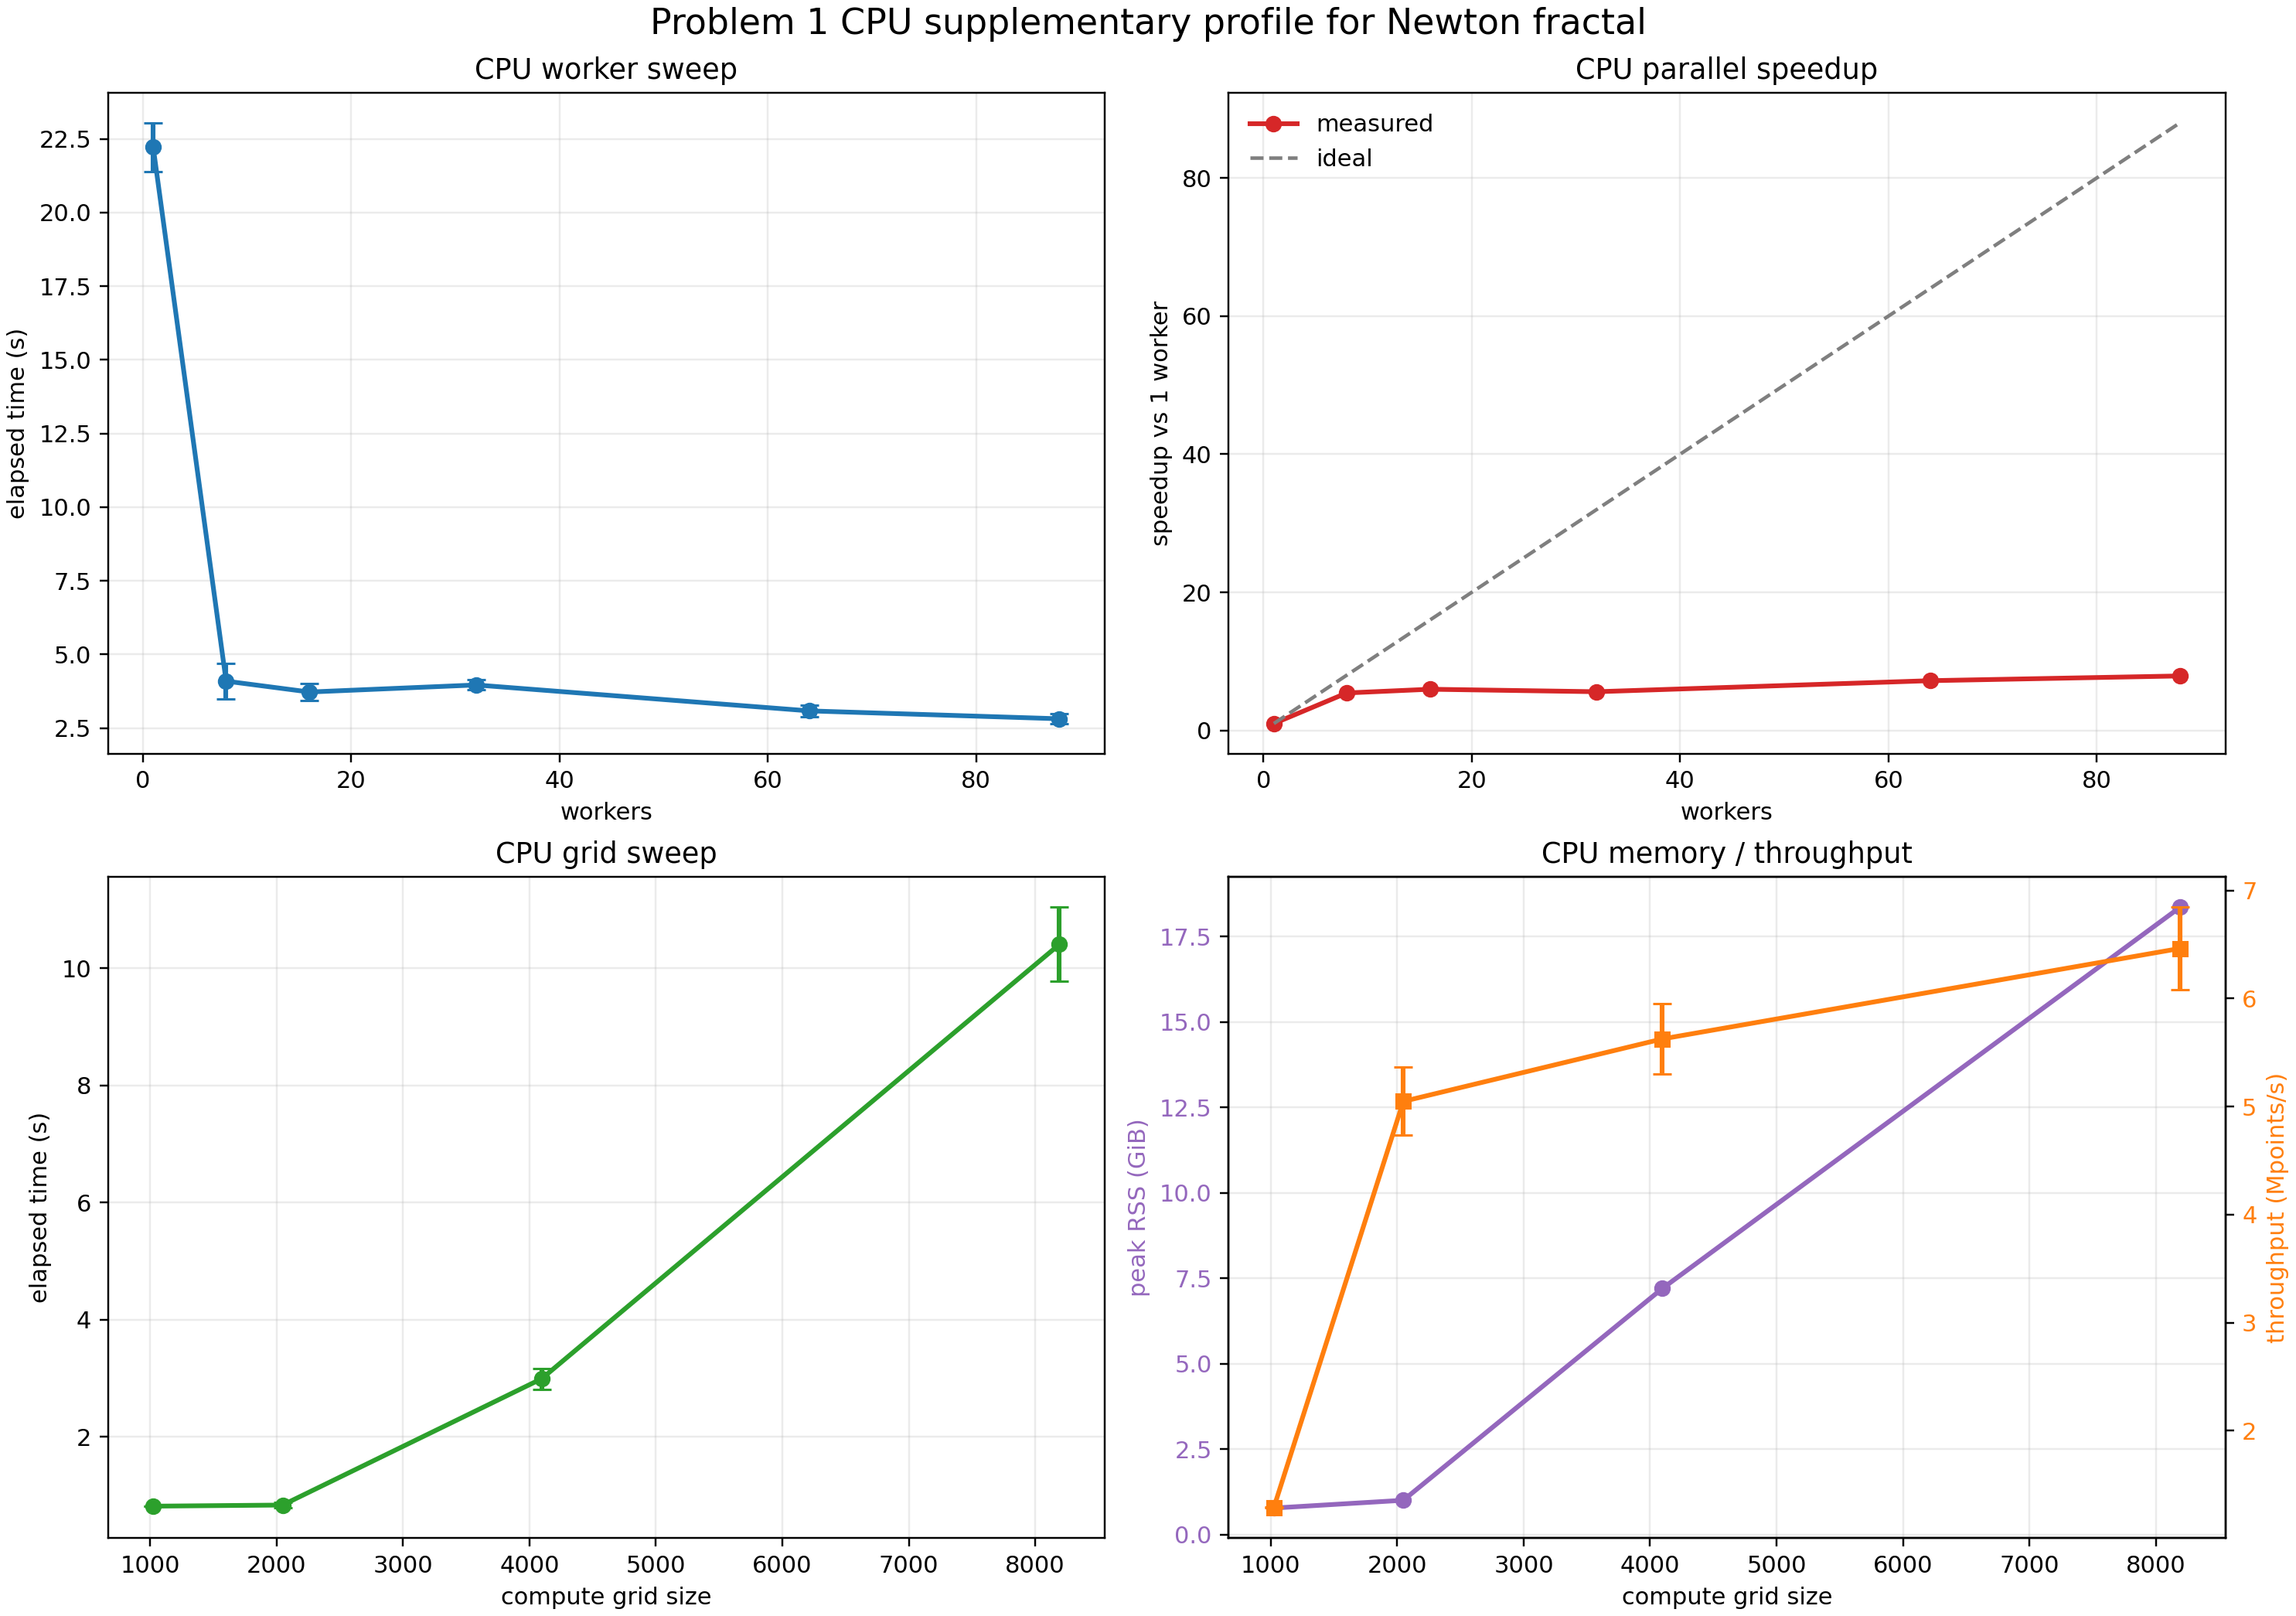
\includegraphics[alt={Problem 1 CPU supplementary profile}]{../../../result/analysis/problem1_cpu_profile.png}
\caption{Problem 1 CPU supplementary profile}
\end{figure}

{\def\LTcaptype{none} % do not increment counter
\begin{longtable}[]{@{}lrrr@{}}
\toprule\noalign{}
CPU 剖面案例 & 耗时 / s（mean ± std） & 吞吐率 / Mpoints/s & 峰值内存 / GiB \\
\midrule\noalign{}
\endhead
\bottomrule\noalign{}
\endlastfoot
\(4096^2\), 1 worker & \(22.22\pm 0.83\) & 0.76 & 3.11 \\
\(4096^2\), 64 workers & \(3.08\pm 0.20\) & 5.46 & 7.14 \\
\(4096^2\), 88 workers & \(2.82\pm 0.16\) & 5.97 & 8.89 \\
\(8192^2\), 64 workers & \(10.41\pm 0.63\) & 6.46 & 18.36 \\
\end{longtable}
}

\analysispart{CPU ultra：流式 tile 聚合和实现边界。}
仅靠原始 Python 多进程主流程，还不足以把 \(80000\times 80000\) 这类极大网格作为附加性能实验来反复测试，因此又补写了一条专用的 CPU ultra 路线。该路线用 C + OpenMP 实现 Newton 直写公式，并结合上半平面对称复用、按输出 tile 流式聚合 \(factor\times factor\) 超采样块，以及常量级小缓冲区而非全平面中间数组。

这里需要明确边界：CPU ultra 属于实现层面的附加优化实验，而不是题面额外要求的标准步骤；它的提速同时依赖 \codeinline{OpenMP} 并行、编译器优化和 tile 参数，而不仅仅来自数学公式本身。该实现的主要目的有两个：其一是把峰值内存从随 \codeinline{compute\_grid} 急剧增长，改为主要受 \codeinline{render\_grid} 和 tile accumulator 大小控制；其二是减少 Python 进程调度和大块临时数组反复分配带来的额外开销。

本轮 CPU ultra benchmark 同样采用 \codeinline{warmup\_runs=1}、\codeinline{timed\_repeats=3}。在 \codeinline{tile\_rows=64} 时，\(20000\)、\(40000\) 和 \(80000\) 三个计算网格的平均耗时分别为 \(13.40\pm 0.02\) s、\(13.97\pm 0.06\) s 和 \(16.48\pm 0.18\) s；峰值 RSS 仍稳定在约 0.118 GiB。进一步对 \(80000\times 80000\) 使用 \codeinline{tile\_rows=256} 复测时，平均耗时降为 \(5.41\pm 0.02\) s，吞吐率达到 1.184 Gpoints/s。历史 final render 摘要中同一 \codeinline{tile\_rows=256} 配置的单次记录为 4.81 s，但正文后续以重复统计表作为更稳健的性能口径。

由此可见，CPU ultra 的关键收益主要来自低内存流式组织和合适的 tile 参数。若把任务明确收缩为 Problem 1 的 Newton 主计算，CPU 侧可以在远低于原始全数组内存压力的条件下完成大网格计算，但这仍应视为对主作业实现的补充，而不是对题面要求本身的改写。

图 3 给出了这条 CPU ultra 路线直接生成的最终 Newton 分形图。这里使用 \(80000\times 80000\) 的计算网格、\(5000\times 5000\) 的输出网格、88 线程和 \codeinline{tile\_rows=256} 的分块设置，既验证了数值分类结果，也说明该路线并不只是统计模式，而是已经能够输出最终可交付图像。

\begin{figure}
\centering
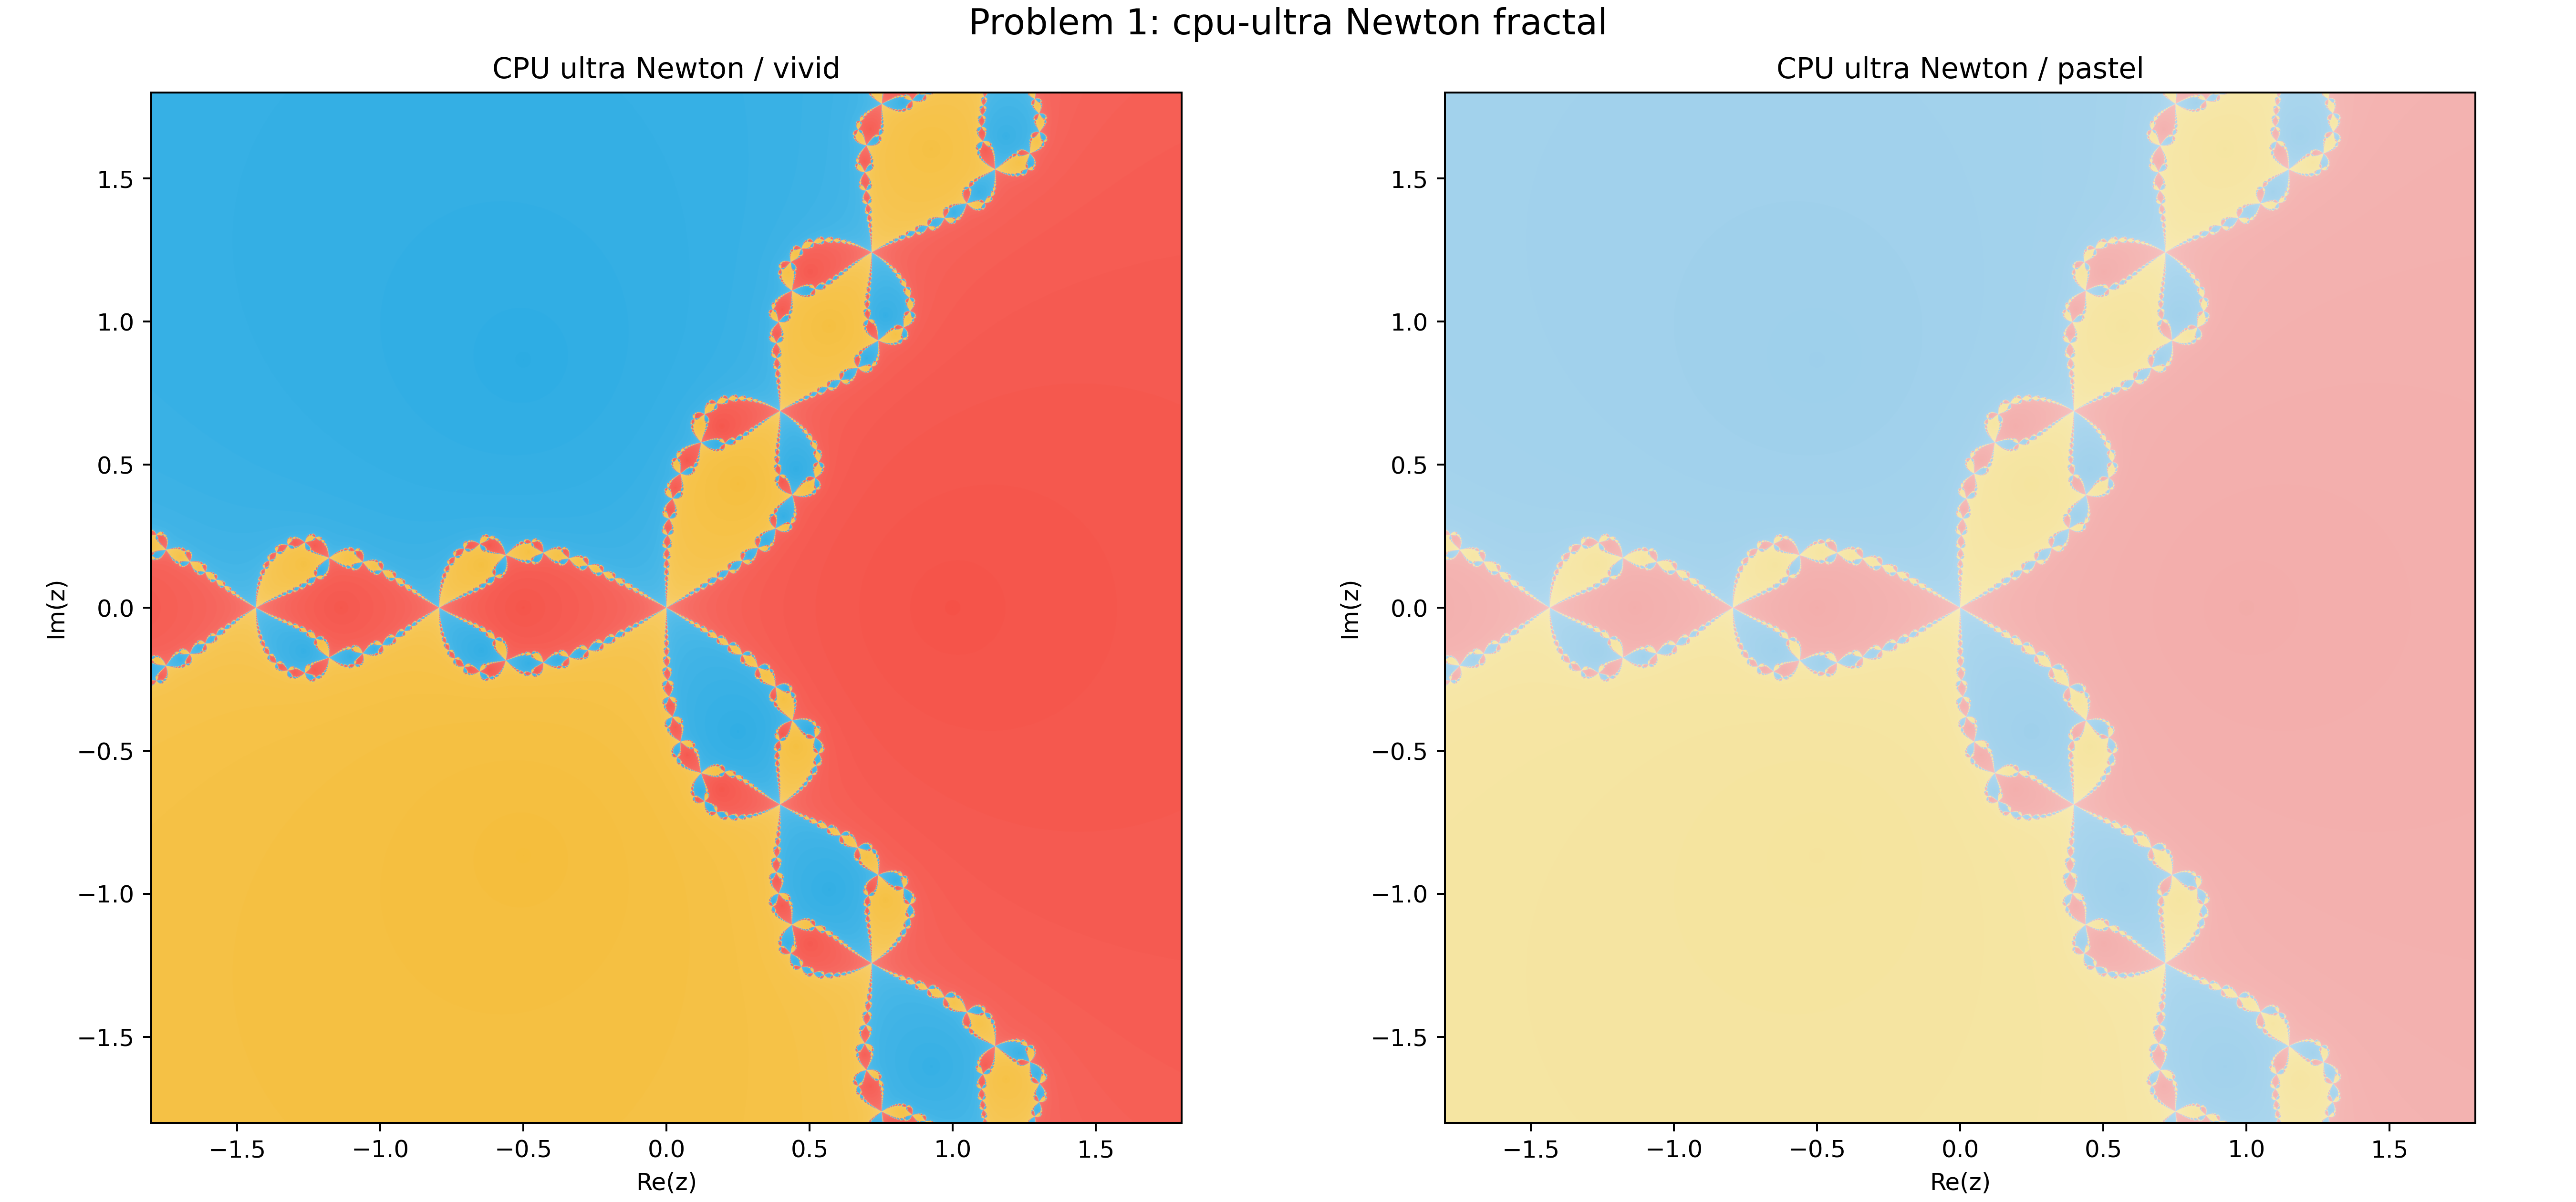
\includegraphics[alt={Problem 1 CPU ultra fractals}]{../../../result/problem1_cpu_ultra_fractals.png}
\caption{Problem 1 CPU ultra fractals}
\end{figure}

{\def\LTcaptype{none} % do not increment counter
\widetabletrue
\begin{longtable}[]{@{}lrrrr@{}}
\toprule\noalign{}
案例 & 耗时 mean ± std / s & 吞吐率 / Gpts/s & RSS / GiB & 收敛比例 \\
\midrule\noalign{}
\endhead
\bottomrule\noalign{}
\endlastfoot
\(20\mathrm{k}\to 5\mathrm{k}\), t64 & \(13.40\pm 0.02\) & 0.030 & 0.118 & 0.999999640000 \\
\(40\mathrm{k}\to 5\mathrm{k}\), t64 & \(13.97\pm 0.06\) & 0.115 & 0.118 & 0.999999601250 \\
\(80\mathrm{k}\to 5\mathrm{k}\), t64 & \(16.48\pm 0.18\) & 0.388 & 0.118 & 0.999999605938 \\
\(80\mathrm{k}\to 5\mathrm{k}\), t256 & \(5.41\pm 0.02\) & 1.184 & 0.118 & 0.999999605938 \\
\end{longtable}
}

若进一步把 \codeinline{cpu-ultra} 的实现写成更具体的算法，它并不是``先生成完整 \(80000\times 80000\) 根标签平面，再整体缩图''，而是把最终 \codeinline{render\_grid}\(\times\)\codeinline{render\_grid} 图像视为细网格块的流式聚合结果。设 \(\mathrm{factor}=\mathrm{compute\_grid}/\mathrm{render\_grid}\)，则输出像素 \((i,j)\) 对应一个 \(\mathrm{factor}\times\mathrm{factor}\) 的细网格块 \(B_{ij}\)。对块内每个采样点，都显式执行 Newton 更新 \[
z_{n+1}=z_n-\frac{z_n^3-1}{3z_n^2}=\frac{2}{3}z_n+\frac{1}{3z_n^2},
\] 若满足 \(\min_k |z_n-r_k|<\tau\)，就记为收敛到第 \(k\) 个根。块内分别统计三个根的命中次数 \(c_0,c_1,c_2\)，再以 \(\arg\max_k c_k\) 作为该输出像素的 basin 标签，并用 \codeinline{iter\_sum}/\codeinline{conv\_count} 记录块内收敛样本的平均迭代步数作为着色强度。由于 \(f(\bar z)=\overline{f(z)}\)，程序只实际计算输出图的上半平面，再把结果按共轭镜像复制到下半平面，同时交换两个非实根的编号。因此，中间态只需要当前 tile 的 \codeinline{count0/count1/count2/iter\_sum/conv\_count} 五个小缓冲区，而不需要保存整张 \codeinline{compute\_grid}\(\times\)\codeinline{compute\_grid} 的根标签数组和步数数组；\codeinline{OpenMP} 仅负责并行外层输出像素循环，Newton 更新、根分类、块内投票和镜像复用都在本实现中显式写出。

\begin{CodeBlock}
for each upper-half tile T do
    allocate count0/count1/count2/iter_sum/conv_count
    parallel for each output pixel (i,j) in T do
        for each fine sample in the factor x factor block B_ij do
            run handwritten Newton iteration and classify the root
            accumulate root counts and iteration sum
        end for
        write argmax-root and mean-iteration to the render buffers
    end for
    flush tile result and free local buffers
end for
mirror the upper-half result to the lower half
\end{CodeBlock}

\clearpage

\analysispart{GPU 与精度扩展：吞吐率不是唯一限制。}
在 CPU 主线和 CPU ultra 已经闭合后，才进一步展开 GPU 与高精度扩展研究。对 \(100000\times 100000\) 网格，\codeinline{complex64} 的 PyTorch 实现耗时 409.53 s，峰值显存 13.10 GiB；同等规模下，Triton 版本仅耗时 3.99 s，峰值显存 5.54 GiB，其收敛比例 \(0.9999996018\)、平均迭代步数 \(6.8143\) 仍与 CPU 主实验统计量保持一致。

这里的意义不在于用 GPU 替代作业本体，而在于说明：当 Problem 1 被扩展到更高采样尺度时，瓶颈已不再只来自 Newton 公式本身，而更取决于复平面采样、数据布局、并行框架和内核组织是否贴近硬件执行方式。

图 4 给出了继续扩大计算网格后的扩展缩放前沿。

\begin{figure}
\centering
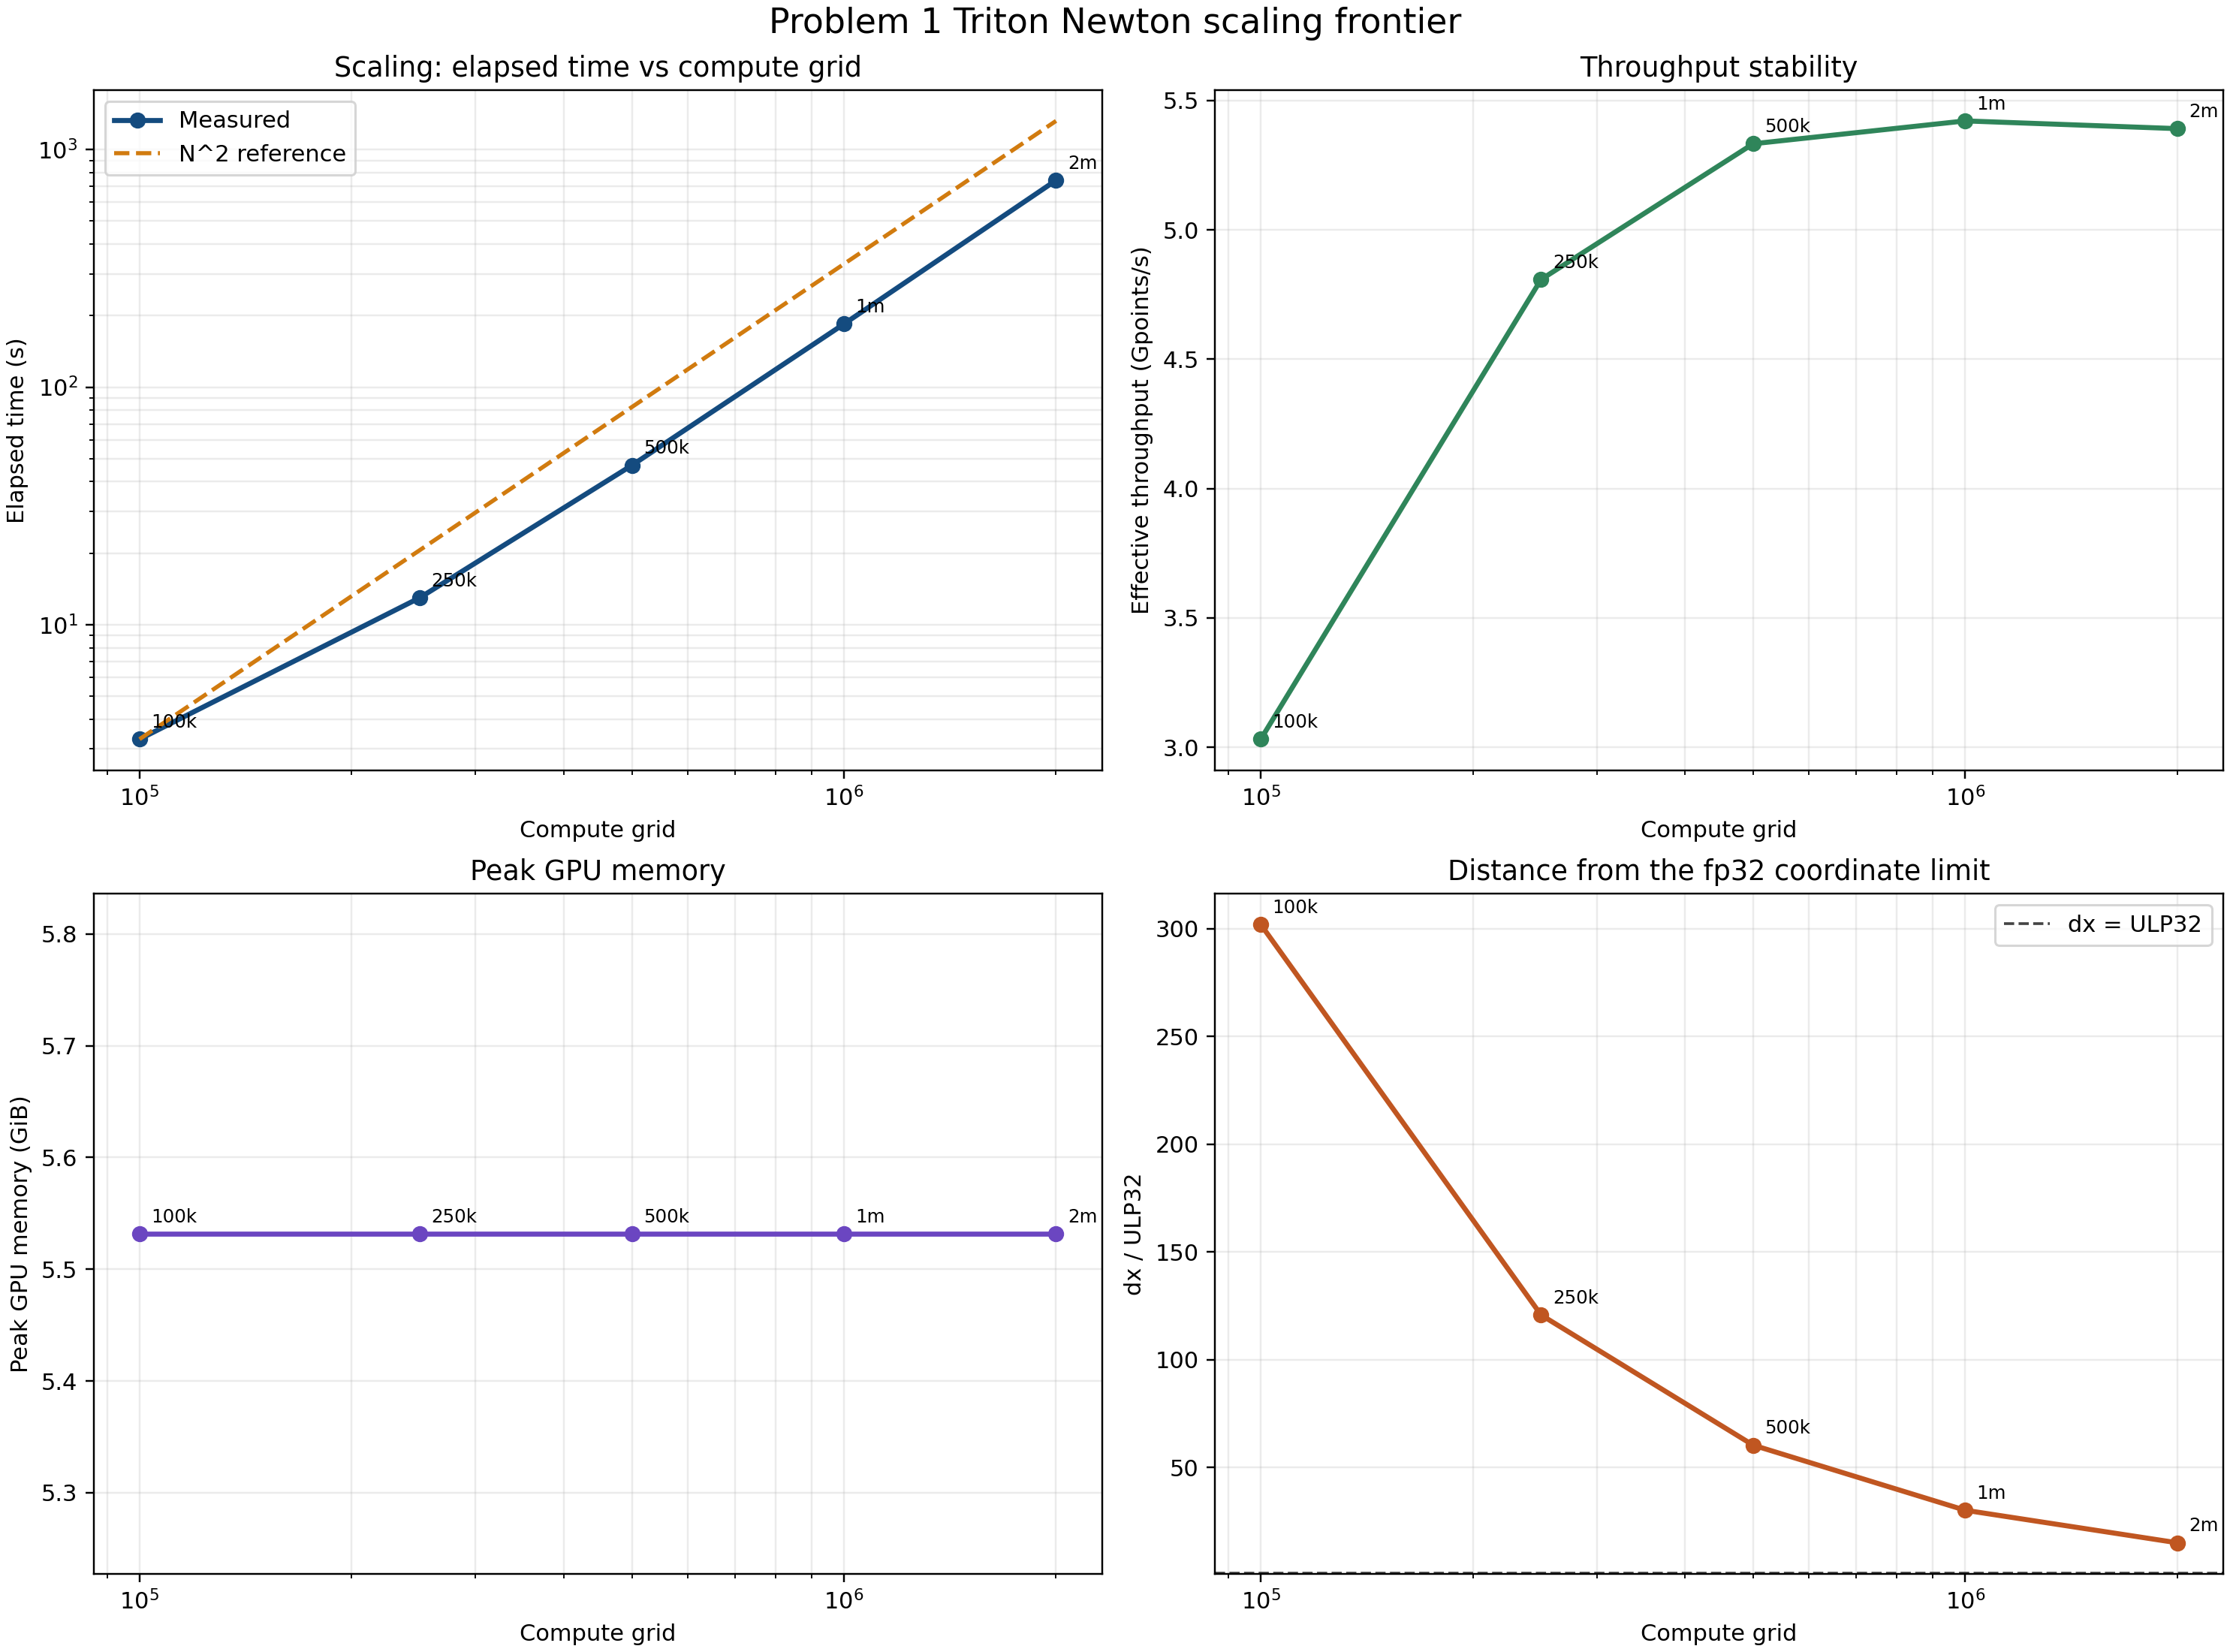
\includegraphics[alt={Problem 1 scaling frontier}]{../../../result/analysis/problem1_scaling_frontier.png}
\caption{Problem 1 scaling frontier}
\end{figure}

由图 4 可见，随着计算网格从 \(100000\) 提升到 \(2000000\)，总耗时由 3.30 s 增加到 741.91 s，总体上仍呈接近平方增长；但吞吐率却从 3.03 Gpoints/s 提升并稳定在 5.39 至 5.42 Gpoints/s 区间，而峰值显存几乎固定在 5.53 GiB。这说明当前 GPU 扩展实现已经通过分块策略把显存占用与全局网格尺度有效解耦，因此继续扩大网格时，主要增加的是总计算时间，而不是显存压力。与此同时，\codeinline{dx / float32 ULP} 的比值从 \(301.99\) 持续下降到 \(15.10\)，表明随着网格变密，单个采样步长正快速逼近 \codeinline{float32} 的可分辨极限；这意味着问题已不再只是``能否算得更快''，而是逐步转化为``在坐标分辨率接近极限时能否保持分类正确''。

图 5 给出了接近 \codeinline{float32} 坐标分辨率上限时的精度前沿。

\begin{figure}[H]
\centering
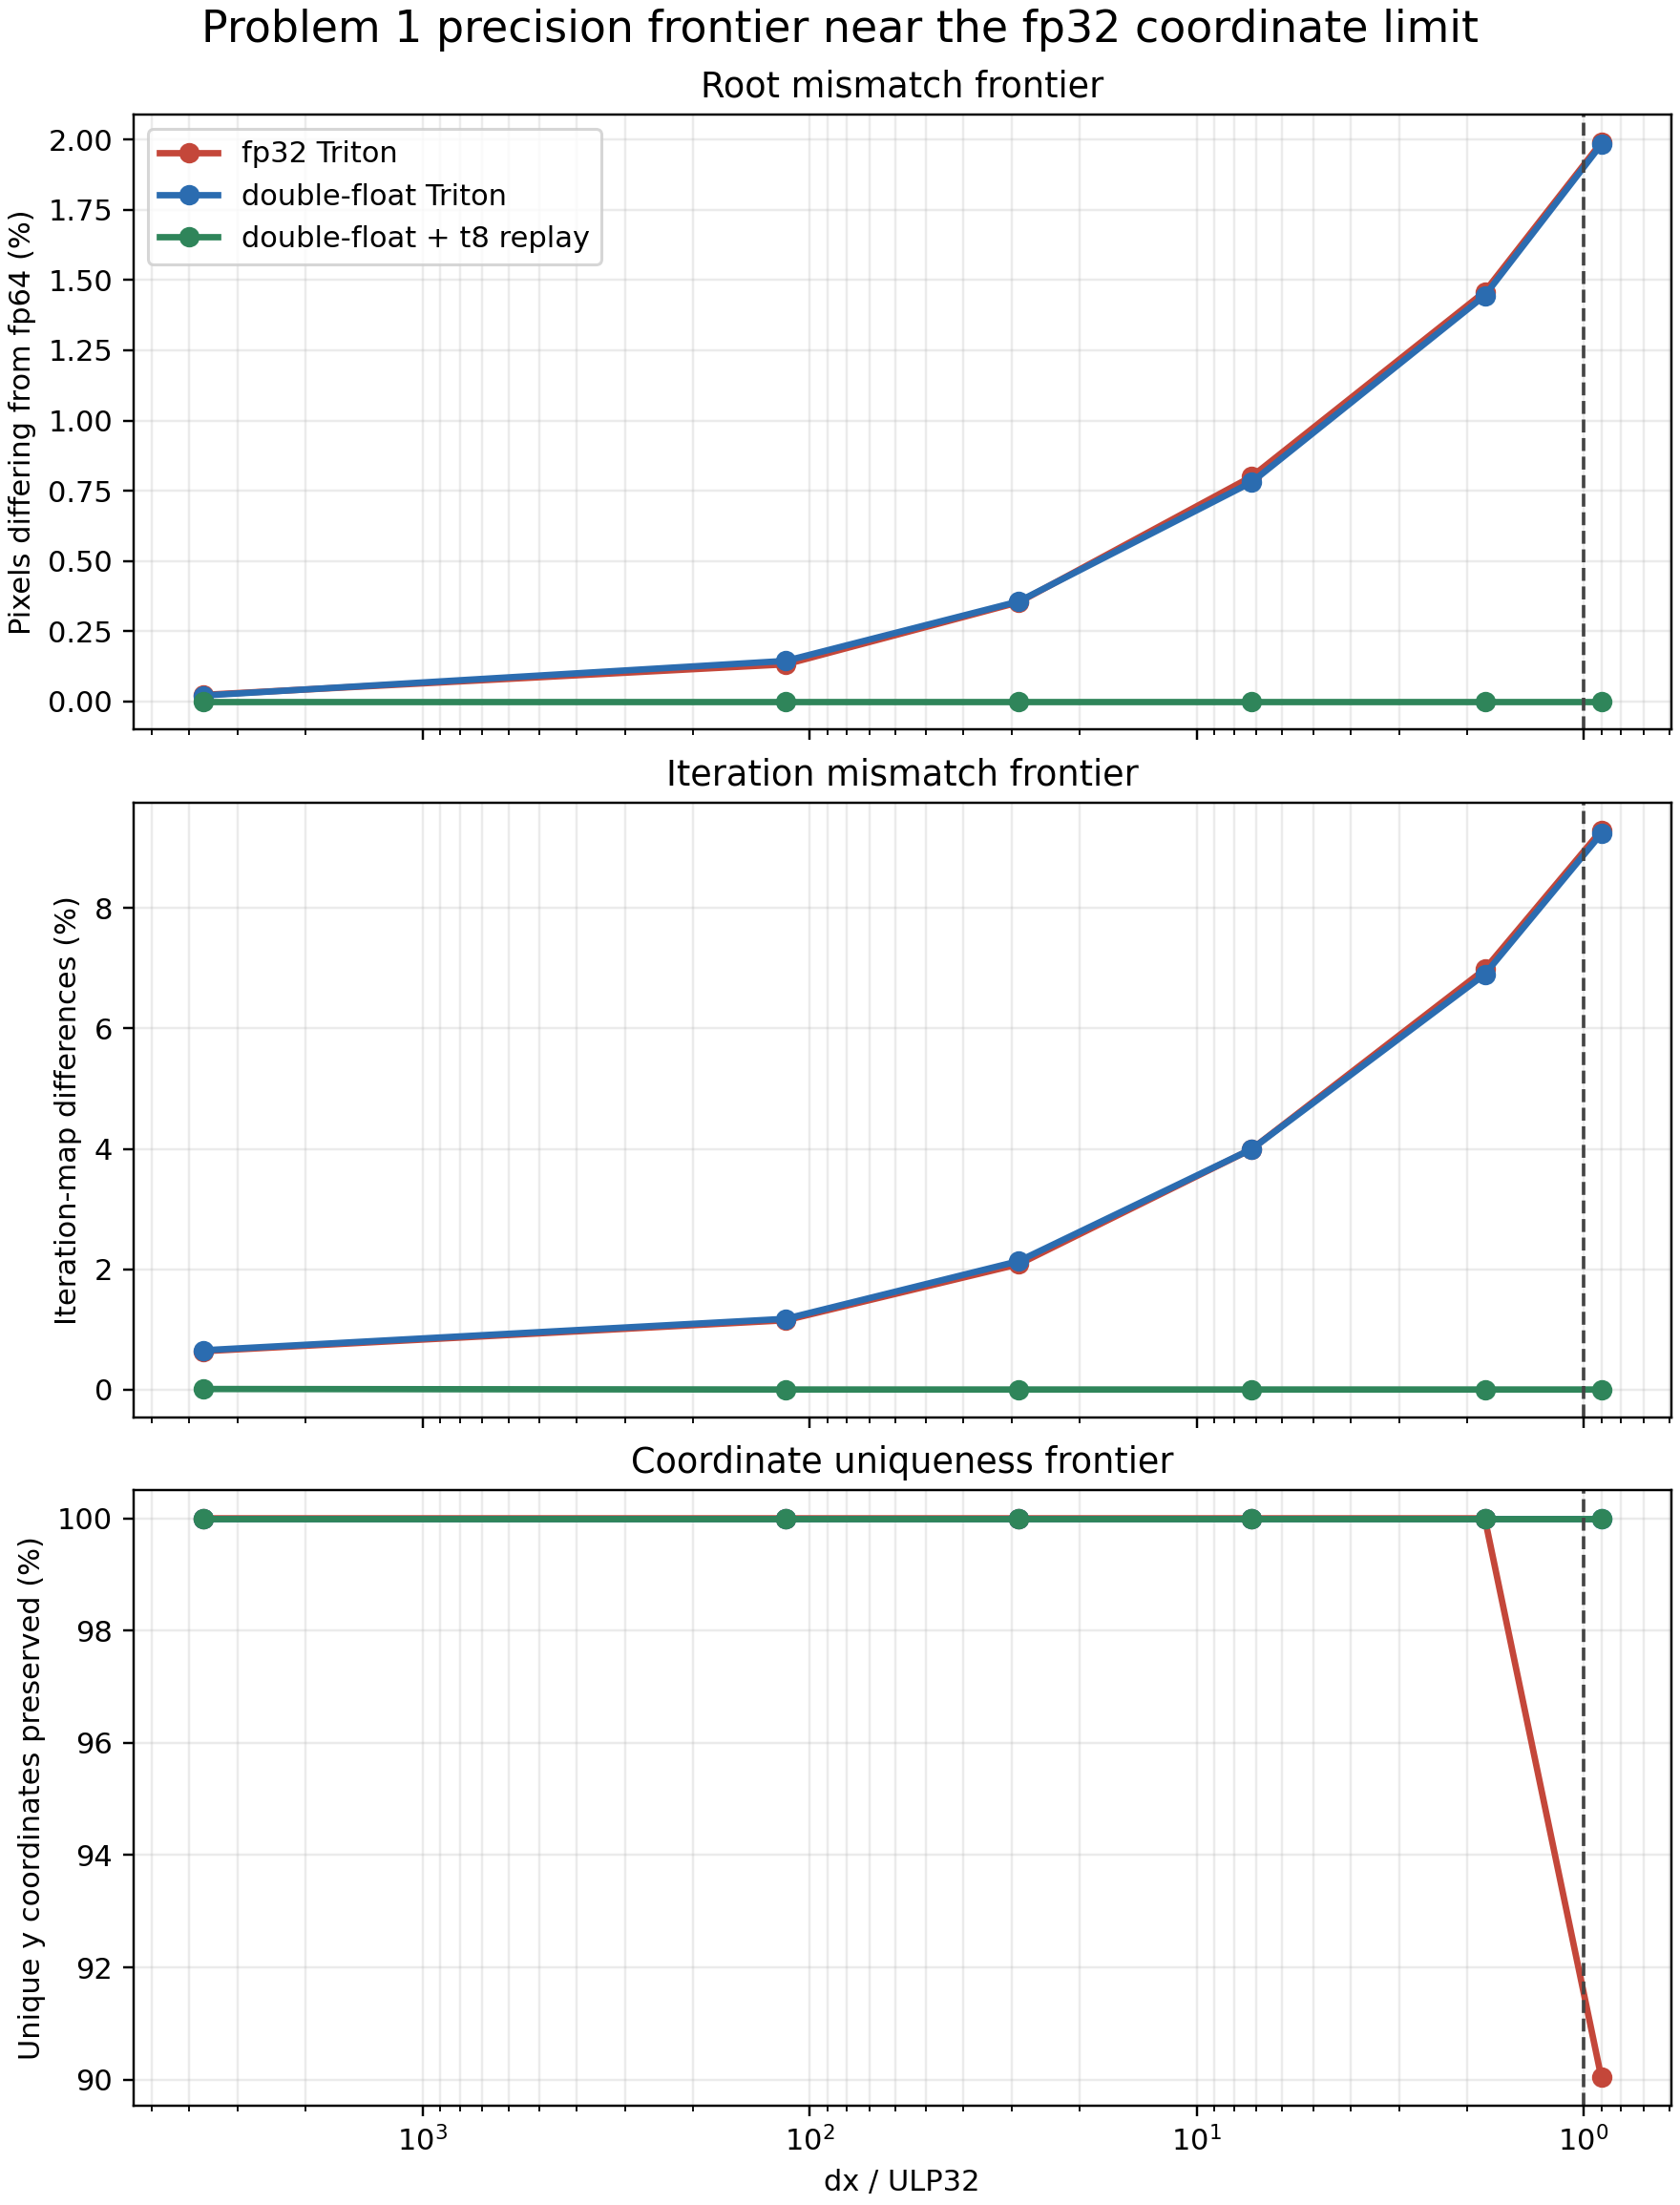
\includegraphics[alt={Problem 1 precision frontier}]{../../../result/analysis/problem1_precision_frontier.png}
\caption{Problem 1 precision frontier}
\end{figure}

由图 5 可见，当全局网格达到 \(33554432\) 时，单点步长仅为 \codeinline{float32} ULP 的 0.9 倍。此时，\codeinline{fp32\_triton} 相对 \codeinline{fp64} 参考已经出现 5217 个像素的根分类差异，占比 \(1.99\%\)；更重要的是，其 \(y\) 方向唯一采样值比例下降到 \(90.04\%\)，说明采样坐标已经发生明显碰撞。即使改用不带 replay 的基础 double-float 实现，仍然存在 5198 个像素的分类偏差，这表明仅仅扩展表示精度并不足以完全消除迭代轨道的偏移。只有在引入 \codeinline{doublefloat\_triton\_t8} 的 replay 机制后，\(8192\) 到 \(33554432\) 全部测试网格才重新与 \codeinline{fp64} 参考保持一致，达到 \codeinline{root\_diff\_vs\_fp64 = 0}，同时 \codeinline{unique\_x\_percent} 与 \codeinline{unique\_y\_percent} 均恢复为 \(100\%\)。

\analysispart{结论边界：主体、优化和扩展三层分开理解。}
综合来看，本题现在可以更准确地分成三层结论。第一层是作业主体：原始 CPU 并行程序已经独立完成 Newton 与 secant 分形图、统计量和其他各题的数值求解。第二层是 CPU 深化优化：针对 Problem 1 的 Newton 主计算，专用的 \codeinline{cpu-ultra} 路线表明，大网格下真正需要解决的是内存组织和分块策略，而不是简单增加 worker 数；一旦把中间态改成流式 tile 聚合，并接受 C + OpenMP + 编译器优化这一实现前提，就可以把同一 Newton 任务做得更紧凑。第三层才是扩展研究：分块 GPU 内核进一步提升了更大网格下的吞吐率，但当采样步长逼近 \codeinline{float32} 分辨率极限时，若没有更高精度坐标表示与 replay 修正机制，最终图像仍会出现系统性漂移。因此，GPU 路线应理解为对 CPU 作业主线的放大与深化，而不是对原始作业求解过程的替代。

\reportgroup{II. Newton-Bisection 混合法求非线性方程根}

\problem{Problem 2：Newton-Bisection 混合法求非线性方程根}

\scriptlink{problem2.py}

\blocktitle{待求问题}

使用完整的 Newton-Raphson 与 Bisection 混合算法，求

\[
f(x)=4\cos x-e^x
\]

的实根。

\blocktitle{解决方式}

本题先扫描变号区间，再在每个括区内执行守护式 Newton-Bisection：

\begin{CodeBlock}
Input : interval [L, R]
Output: all roots in [L, R]

scan [L, R] and collect sign-change brackets [a, b]
for each bracket [a, b] do
    x <- (a + b) / 2
    repeat
        x_newton <- x - f(x) / f'(x)
        if a < x_newton < b then
            x_next <- x_newton
        else
            x_next <- (a + b) / 2
        end if
        update bracket so that f(a) f(b) <= 0
        x <- x_next
    until convergence
end for
\end{CodeBlock}

本报告固定研究区间为 \([-10,2]\)，从而把``所有负根''的开放任务转化为有限区间内的可验证求根问题。

\blocktitle{问题答案}

在 \([-10,2]\) 内共得到 4 个根，如表 2 所示。

{\def\LTcaptype{none} % do not increment counter
\begin{longtable}[]{@{}lrrrr@{}}
\toprule\noalign{}
括区 & 根 & 步数 & 残差 & 绝对误差 \\
\midrule\noalign{}
\endhead
\bottomrule\noalign{}
\endlastfoot
\([-7.854,-7.852]\) & -7.853884573753 & 3 & 3.119e-16 & 0 \\
\([-4.716,-4.714]\) & -4.714629778215 & 3 & -3.296e-16 & 0 \\
\([-1.516,-1.514]\) & -1.515864122805 & 3 & -7.216e-16 & 2.220e-16 \\
\([0.904,0.906]\) & 0.904788217873 & 3 & -1.776e-15 & 2.220e-16 \\
\end{longtable}
}

因此，在选定区间内的全部实根已经被完整求出，且都与高精度参考值在双精度舍入误差范围内一致。

\blocktitle{分析}

本题的关键并不是单纯``用 Newton 找根''，而是利用括区信息保持算法稳定性。若 Newton 切线步跳出括区，就立即回退到二分步，从而保证 \(f(a)f(b)\le 0\) 的不变量始终成立。该策略兼顾了 Newton 的快速局部收敛和二分法的全局可靠性。

\reportgroup{III. 带参数方程的 Müller-Brent 求根}

\problem{Problem 3：带参数方程的 Müller-Brent 求根}

\scriptlink{problem3.py}

\blocktitle{待求问题}

求下列两个函数的根：

\[
f(x)=x\tan x-\sqrt{h^2-x^2},
\qquad
g(x)=x\cot x+\sqrt{h^2-x^2},
\]

其中 \(h\) 取若干代表性数值，例如 \(0.2\)、\(0.5\)、\(1.0\) 与 \(2.0\)。

\blocktitle{解决方式}

算法组织如下：

\begin{CodeBlock}
Input : parameter h and target function phi(x)
Output: all admissible roots for this h

restrict domain to (0, h)
split domain by singularities of tan or cot
for each valid subinterval do
    if sign change is detected then
        apply Brent-style safeguarded iteration
        record converged root
    end if
end for
if no sign change is found in all subintervals then
    report no root
end if
\end{CodeBlock}

这里先处理定义域约束 \(x<h\)，再按 \(\tan\) 或 \(\cot\) 的奇点分段，否则根搜索将失去意义。

\blocktitle{问题答案}

结果如表 3 所示。

{\def\LTcaptype{none} % do not increment counter
\begin{longtable}[]{@{}lll@{}}
\toprule\noalign{}
(h) & (f(x)) 的根 & (g(x)) 的根 \\
\midrule\noalign{}
\endhead
\bottomrule\noalign{}
\endlastfoot
0.2 & 0.19616428118784215 & 无根 \\
0.5 & 0.45018361129487355 & 无根 \\
1.0 & 0.7390851332151607 & 无根 \\
2.0 & 1.029866529322259 & 1.8954942670339807 \\
\end{longtable}
}

所有已求得的根，其残差均处于 \(10^{-15}\) 量级或更小。

\blocktitle{分析}

本题的主要困难来自``定义域 + 奇点 + 非线性''三者同时存在。对 \(g(x)\) 而言，较小的 \(h\) 会显著压缩可行区间，因此在 \(h=0.2\)、\(0.5\) 和 \(1.0\) 时未检测到根；只有当 \(h\) 增大到 \(2.0\) 时，函数结构才允许实根出现。这说明参数 \(h\) 不仅改变根的位置，还可能直接改变根的存在性。

当 \(h=1.0\) 时，\(f(x)\) 的根约为 \(0.7390851332\)，它与经典方程 \(x=\cos x\) 的解一致，因此也构成了额外的正确性核验。

\reportgroup{IV. 范盛金公式求三次方程的根}

\problem{Problem 4：范盛金公式求三次方程的根}

\scriptlink{problem4.py}

\blocktitle{待求问题}

使用范盛金公式求解

\[
x^3-70.5x^2+1533.54x-10082.44=0
\]

的三个实根。

\blocktitle{解决方式}

求解流程如下：

\begin{CodeBlock}
Input : cubic coefficients A, B, C
Output: three real roots and residuals

transform x = y - A / 3
compute depressed-cubic parameters p and q
compute theta from arccos formula
for k in {0, 1, 2} do
    y_k <- 2 * sqrt(-p / 3) * cos((theta + 2k pi) / 3)
    x_k <- y_k - A / 3
end for
evaluate residuals of original polynomial
\end{CodeBlock}

在本题中，降次后得到的 \(q\) 非常接近 \(0\)，因此三根结构具有明显的对称性。

\blocktitle{问题答案}

程序输出如下。

{\def\LTcaptype{none} % do not increment counter
\begin{longtable}[]{@{}lr@{}}
\toprule\noalign{}
根 & 残差 \\
\midrule\noalign{}
\endhead
\bottomrule\noalign{}
\endlastfoot
12.40000000000002 & 3.637978807091713e-12 \\
23.499999999999954 & 5.4569682106375694e-12 \\
34.60000000000002 & 1.8189894035458565e-12 \\
\end{longtable}
}

因此，可将最终答案写为

\[
x=12.4,\quad 23.5,\quad 34.6.
\]

\blocktitle{分析}

降次变换后得到

\[
y^3-123.21y-5.457\times 10^{-12}=0,
\]

其中常数项已经极小，因此方程几乎退化为

\[
y(y^2-123.21)=0.
\]

这正是三个实根近似等于 \(0\) 与 \(\pm 11.1\) 的原因。数值残差仅剩 \(10^{-12}\) 量级，说明当前误差主要来自浮点舍入，而不是范盛金公式失效。

\reportgroup{V. 地月系统的 L1 点}

研究地月系统中的 \(L_1\) 点。题目包含以下两个子问：

\begin{enumerate}
\def\labelenumi{\arabic{enumi}.}
\tightlist
\item
  证明距离地心为 \(r\) 的平衡点满足
\end{enumerate}

\[
\frac{GM}{r^2}-\frac{Gm}{(R-r)^2}=\omega^2r.
\]

\begin{enumerate}
\def\labelenumi{\arabic{enumi}.}
\setcounter{enumi}{1}
\tightlist
\item
  利用 Newton 方法或 secant 方法求出 \(r\) 的数值解，并至少给出四位有效数字。
\end{enumerate}

\problem{Problem 5(a)：平衡方程推导}

\scriptlink{problem5.py}

\blocktitle{解决方式}

设待求平衡点位于地月连线上，距地心为 \(r\)，距月心为 \(R-r\)，并与月球一起以角速度 \(\omega\) 作同步转动。沿地月连线取指向地球的方向为正，则试探质点受到的两个引力加速度分别为

\[
a_E=\frac{GM}{r^2},\qquad
a_M=-\frac{Gm}{(R-r)^2}.
\]

这里 \(a_E\) 指向地球，\(a_M\) 指向月球，因此在所选正方向下二者符号相反。若该点能够与月球保持同角速度转动，则质点必须具有指向地球的向心加速度

\[
a_c=\omega^2 r.
\]

于是平衡条件就是沿地月连线方向的合加速度恰好等于所需向心加速度，即

\[
a_E+a_M=a_c.
\]

代入上式可得

\[
\frac{GM}{r^2}-\frac{Gm}{(R-r)^2}=\omega^2r,
\]

这正是题目第 (a) 问所要求的平衡关系。

\blocktitle{问题答案}

由地球引力、月球引力与同步转动所需向心加速度的平衡关系，可直接得到

\[
\frac{GM}{r^2}-\frac{Gm}{(R-r)^2}=\omega^2r.
\]

其中左端是沿地月连线方向的净引力加速度，右端是半径为 \(r\) 的同步圆周运动所需向心加速度，因此该式具有明确的物理含义。

\blocktitle{分析}

\(L_1\) 点位于地月之间且更靠近月球，这是因为只有在靠近月球处，月球引力才足以显著抵消地球引力，使卫星获得恰好满足同步转动所需的向心加速度。Newton 与 secant 在不同初值下都快速收敛到同一解，说明本题所对应的标量方程在合理初值附近具有良好的数值可解性。

\problem{Problem 5(b)：数值求解流程}

\scriptlink{problem5.py}

\blocktitle{解决方式}

将第 (a) 问得到的平衡方程写为

\[
\frac{GM}{r^2}-\frac{Gm}{(R-r)^2}=\omega^2r,
\]

等价地定义

\[
F(r)=\frac{GM}{r^2}-\frac{Gm}{(R-r)^2}-\omega^2r.
\]

对 Newton 方法还需要导数

\[
F'(r)=-\frac{2GM}{r^3}-\frac{2Gm}{(R-r)^3}-\omega^2.
\]

计算过程如下：

\begin{CodeBlock}
Input : physical constants G, M, m, R, omega
Output: numerical root r of the L1 equation

define F(r) = GM / r^2 - Gm / (R - r)^2 - omega^2 r
derive F'(r) for Newton iteration

Newton:
    choose initial guess r0
    iterate r_{n+1} = r_n - F(r_n) / F'(r_n)

Secant:
    choose two initial guesses r0, r1
    iterate with secant update

compare both results with high-precision reference
\end{CodeBlock}

其中，方程的物理含义是：地球引力提供向心趋势，月球引力抵消其中一部分，因此平衡点位于地球与月球之间。

\blocktitle{问题答案}

利用 Newton 与 secant 方法求得的数值结果如下。

{\def\LTcaptype{none} % do not increment counter
\widetabletrue
\begin{longtable}[]{@{}llrrrr@{}}
\toprule\noalign{}
方法 & 初值 & (r) / m & 步数 & 残差 & 绝对误差 \\
\midrule\noalign{}
\endhead
\bottomrule\noalign{}
\endlastfoot
Newton & \(3.2\times 10^8\) & 326045071.665355 & 5 & -1.735e-18 & 0 \\
Secant & \((3.0\times 10^8,\ 3.3\times 10^8)\) & 326045071.665355 & 6 & -1.735e-18 & 0 \\
\end{longtable}
}

因此，

\[
r=326045071.66535544\ \mathrm{m}
\approx 3.260\times 10^8\ \mathrm{m}.
\]

若进一步换算，则

\[
\frac{r}{R}\approx 0.84819,\qquad
R-r\approx 5.835\times 10^7\ \mathrm{m}.
\]

\blocktitle{分析}

\(L_1\) 点位于地月之间且更靠近月球，这是因为只有在靠近月球处，月球引力才足以显著抵消地球引力，使卫星获得恰好满足同步转动所需的向心加速度。Newton 与 secant 在不同初值下都快速收敛到同一解，说明本题所对应的标量方程在合理初值附近具有良好的数值可解性。

\end{document}
